\subsection{Cloud-proximity phenomenology}
\label{sec:result-cld_dist}

% Lead with the observation:

% - XCO2 anomaly versus cloud distance;
% - positive near-cloud response over land and negative response over ocean;
% - characteristic land-r15 and ocean-r05 distance scales;
% - quality-flag composition and observation loss with cloud distance.

% This result establishes the problem before introducing correction skill.

We analyze the $17.75$M footprints from the 2016-2020 analysis set (Sect.~\ref{sec:method-daataset-split}) with a valid nearest cloud distance. $41.7\%$ of all footprints lie within 4 km of the nearest detected cloud ($60.7\%$ within 10 km). We use $d_0 = 10$~km as the reference to calculate the \xcobc anomaly ($\Delta \mathrm{X_{CO2}^{B11}}$), as shown in Fig.~\ref{fig:OCO-ocean-land-cld_dist}a. The results demonstrate that $\Delta \mathrm{X_{CO2}^{B11}}$ is opposite in sign, with negative over ocean and positive over land before any correction is applied. Furthermore, the ocean response has decayed by $\thicksim5$ km, well inside the threshold, whereas the land response is still $\thicksim0.5$ ppm when the 10-km reference cut truncates it by construction. In other words, the cloud-influence distance could be different over ocean and land. As a result, we set the new reference distances separately with $d_0 = 5$~km for ocean and $d_0 = 15$~km for land.



\begin{figure}[t]
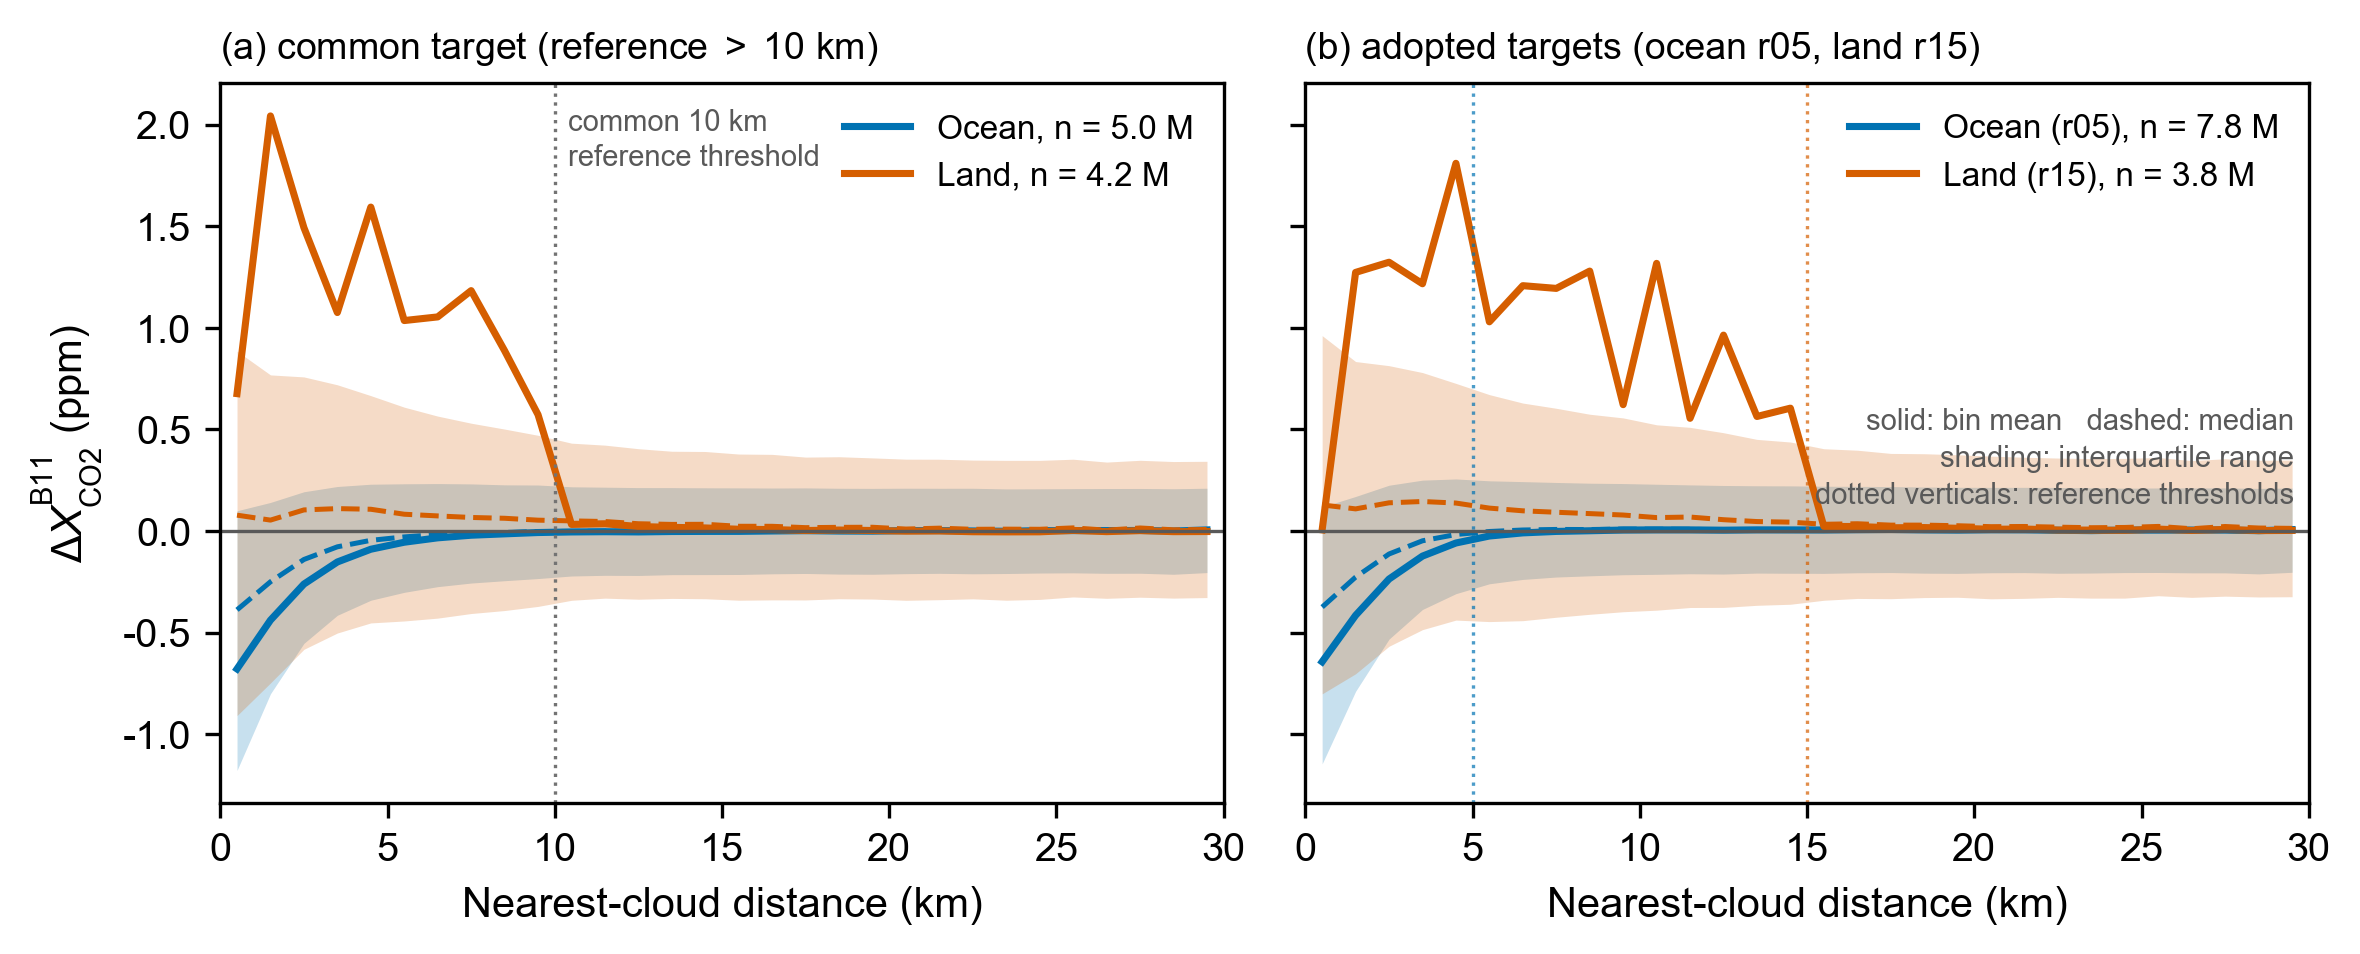
\includegraphics[width=\textwidth]{figures/fig03_anomaly_decay.png}
\caption{Within-orbit clear-sky \xco anomaly versus nearest-cloud distance for the 2016–2020 analysis set (116 dates; 1-km bins). (a) Both surfaces under a common anomaly target whose clear-sky reference lies beyond 10 km. The common threshold is too tight for land and unnecessarily wide for ocean, motivating the surface-specific radii. (b) The adopted production targets with ocean referenced beyond 5 km (r05, n = 7.8 M) and land beyond 15 km (r15, n = 3.8 M). Solid lines show the bin mean, dashed lines the median, and shading the interquartile range: over ocean the whole distribution shifts negative near cloud, whereas over land the mean far exceeds the nearly unmoved median. The land bias is carried by a skewed tail of strongly affected soundings rather than a shift of the full population.}
\label{fig:OCO-ocean-land-cld_dist}
\end{figure}


After recalculating $\Delta \mathrm{X_{CO2}^{B11}}$, the land response indeed persists to $\thicksim15$ km, and the ocean curve is unchanged (Fig.~\ref{fig:OCO-ocean-land-cld_dist}b). The dotted lines mark each reference threshold, beyond which the anomaly returns to zero by construction. The signature of opposite sign of ocean and land $\Delta \mathrm{X_{CO2}^{B11}}$ also remains the same. 59.1\% of ocean footprints are within the 5 km ocean target radius, and 46.8\% of land footprints are within the 15 km land target radius. We use the newly calculated $\Delta \mathrm{X_{CO2}^{B11}}$ with $r05$ for ocean and $r15$ for land in later analysis and training.